\tikzsetfigurename{module2_1_16_poolcoordinaten3}
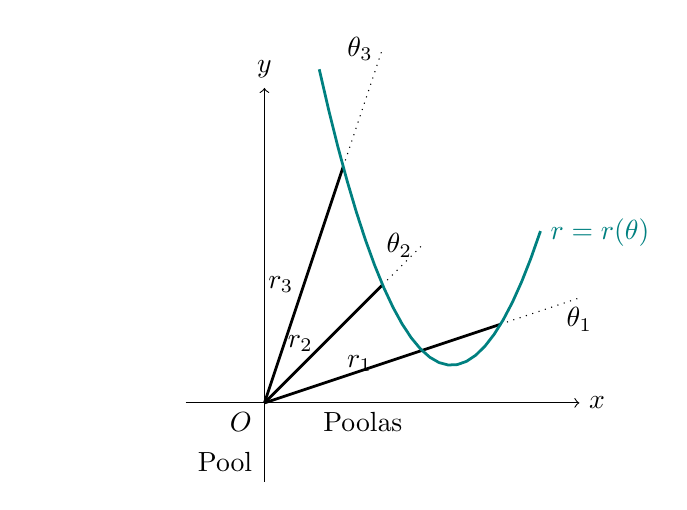
\begin{tikzpicture}

\coordinate (a) at (0,0) node[anchor=south,below,xshift=-0.3cm]{$O$};
\coordinate (a) at (0,0) node[anchor=south,below,xshift=-0.5cm,yshift=-0.5cm]{Pool};
\coordinate (b) at (1,0);
\coordinate (c) at (2.5,3);

\draw[thin,gray!40] (-3,-1) (3,3);
\draw[->] (-1,0)--(4,0) node[right]{$x$};
\draw[->] (0,-1)--(0,4) node[above]{$y$};
%\draw[line width=2pt,black,-stealth](0,0)--(2,0) node[anchor=south,xshift=0.3cm]{$\vec{e_x}$};
%\draw[line width=2pt,black,-stealth](0,0)--(0,2) node[anchor=south,xshift=0.3cm]{$\vec{e_y}$};


\draw[-] (0,0)--(2.5,0) node[anchor=south,below,midway]{Poolas};

\draw[line width=1pt](0,0)--(1,3) node[anchor=south,left,midway]{$r_3$};
\draw[dotted] (1,3)--(1.5,4.5) node[anchor=north,left]{$\theta_{3}$};
\draw[line width=1pt](0,0)--(1.5,1.5) node[anchor=south,left,midway]{$r_2$};
 \draw[dotted] (1.5,1.5)--(2,2) node[anchor=north,left]{$\theta_{2}$};
\draw[line width=1pt](0,0)--(3,1) node[anchor=south,left,midway]{$r_1$};
 \draw[dotted] (3,1)--(4,4/3) node[anchor=north]{$\theta_{1}$};

\draw[teal,cap=rect,line width=1, opacity=1, domain=0.7:3.5] plot (\x, {
	4/3*pow(\x,2)-19/3*pow(\x,1)+8  		% <- plaats het functievoorschrift hier
}) node[right,opacity=1]{$r=r(\theta)$};

%\coordinate (d) at (2,2.4) node[anchor=south]{$P$}

%\path[clip] (0.866,0.5) -- (0,0) -- (0.866,0) -- cycle;
%\node[circle,draw=black,minimum size=40pt] at (0,0) (circ) {};
%\draw[blue] (1cm,0cm) arc (90:125:0.5cm);

%  \draw
%(3,-1) coordinate (a) node[right] {a}
%-- (0,0) coordinate (b) node[left] {b}
%-- (2,2) coordinate (c) node[above right] {c}
%pic["$\alpha$",draw=orange,<->,angle eccentricity=1.2,angle radius=1cm] {angle=a--b--c};

%\pic [draw, ->, "$\theta$", angle eccentricity=1.5] {angle = b--a--c};


%\draw[line width=2pt,blue,-stealth](0,0)--(-0.5,$\sqrt{3}/2$) node[anchor=south]{$\vec{e_v}$};

\end{tikzpicture}